\documentclass[usenames,dvipsnames]{beamer}
\usetheme{Boadilla}
\usepackage{amsmath}
\usepackage{amsthm}
\usepackage{amssymb}
\usepackage{amsfonts}
\usepackage{mathtools}
\usepackage{wrapfig}
\usepackage{bm}
\usepackage{float}
\usepackage{tikz}
\usetikzlibrary {patterns}
\usepackage[normalem]{ulem}
\usepackage[export]{adjustbox}
\usepackage{dcolumn}
\usepackage{multirow}
\usepackage{ctable}
\usepackage{etoolbox}
\usepackage{xcolor}

\usepackage{newfloat,algcompatible}
\usepackage{subcaption}
\captionsetup[subfigure]{justification   = raggedright, singlelinecheck=false}
\captionsetup[subfigure]{labelformat=empty}

\AtBeginEnvironment{algorithm}{\noindent\hrulefill\par\nobreak\vskip-5pt}

\DeclareMathOperator{\Ham}{\mathcal{H}}
\DeclareMathOperator{\avg}{\mathop{\mathbb{E}}}
\newcommand{\floor}[1]{\mathop{\lfloor{#1}\rfloor}}
\newcommand{\Var}{\mathop{\mathrm{Var}}}
\newcommand{\ola}[1]{\overleftarrow{#1}}
\newcommand{\ora}[1]{\overrightarrow{#1}}
\newcommand{\bs}[1]{\boldsymbol{#1}}
%\newtheorem{theorem}{Theorem}

% Define keyword and construction of \RETURN
\algnewcommand\algorithmicreturn{\textbf{return}}
\algnewcommand\RETURN{\State \algorithmicreturn}

\title{Assistant in Computational Biology}
\subtitle{Postdoctoral Research}
\author{Roozbeh H. Pazuki (He/Him)}
%\institute{Imperial College London}
\date{\today}

\setbeamerfont{block body}{size=\tiny}

\begin{document}

\frame{\titlepage}

\setbeamerfont{block body}{size=\small}
\begin{frame}
 \frametitle{GNNs Embeddings}
\begin{block}{Details}
	\begin{itemize}
		\item \textbf{Method Name:} GraphDTA.
		\item \textbf{Publication Year:} 2021.
		\item \textbf{Publication Title:} ``GraphDTA: predicting drug–target binding affinity with  graph neural networks'' \cite{btaa921}.
		\item \textbf{Architectures:} Graph Isomorphism Convolution Network.
		\item \textbf{File Name:} ``drug\_GraphDTA\_GINConvNet\_label.csv''.
	\end{itemize}
\end{block}
\begin{columns}[b]
 \column{0.48\textwidth}
 \centering
		
\column{0.04\textwidth}

 \column{0.48\textwidth}
 \centering
 \end{columns} 
\end{frame}

\setbeamerfont{block body}{size=\tiny}

\begin{frame}
	\frametitle{GNNs Embeddings}
	\begin{block}{Original Model}
	Embedding representations are extracted using the graph isomorphism network (GIN) architecture from \cite{btaa921}. Here, the drug's SMILES alongside 1D convolutional mapping of protein sequences are embedded, and downstream, the drug-target affinity's value is estimated. We trained the model by using the paper's supplementary material.
	\end{block}

	\begin{figure}
		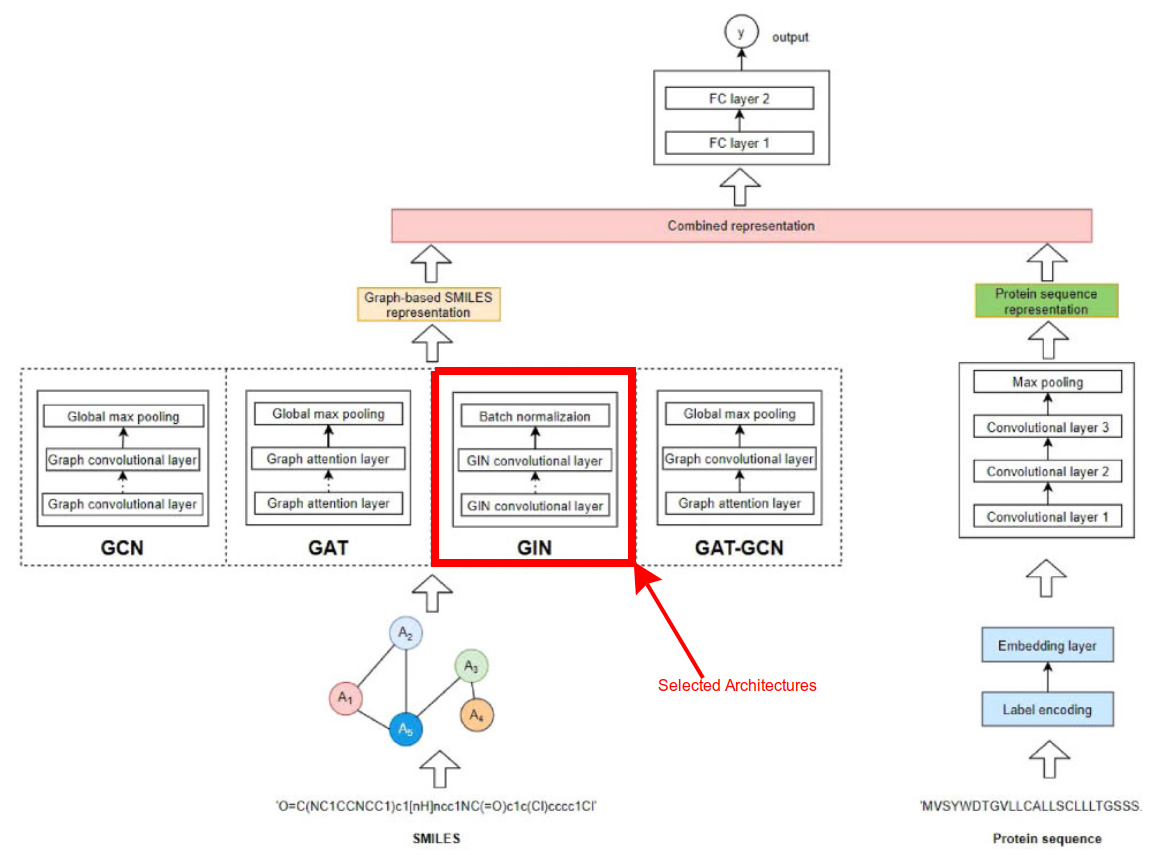
\includegraphics[width=.7\textwidth]{train_workflow}
	\end{figure}
\end{frame}

\begin{frame}
	\frametitle{GNNs Embeddings}
	\begin{block}{Prepration}
     Using the ``rdkit library'', a custom code sanitises and converts SMILES to their graph representations. For each node's atom, the node features were also extracted. Then, by feeding the augmented partial network from \cite{btaa921}, we only use the embedded graphs output.     
     \newline
     \newline     
     
    \textbf{Note:} Ten SMILES string had ``explicit valence'' error, so, are missed on the final embedding.
	\end{block}
	
	\begin{figure}
		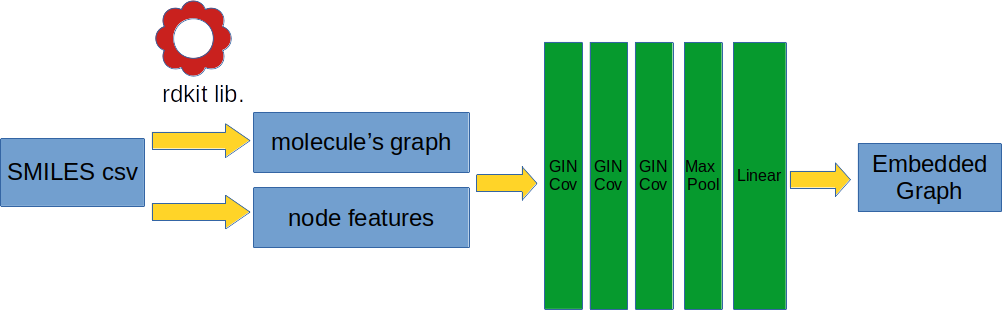
\includegraphics[width=1.0\textwidth]{arch}
	\end{figure}
\end{frame}

\begin{frame}
	\frametitle{GNNs Embeddings}
	\begin{block}{Improvment}
		Investigating the 2D tSNE projection of the embedded space, we realise that the batch normalisation layers are fixed for different populations on the original trained network (left Fig.). After updating the model for the task's molecules, we will see communities in the embedding space (right Fig.).
	\end{block}
	
	\begin{figure}
		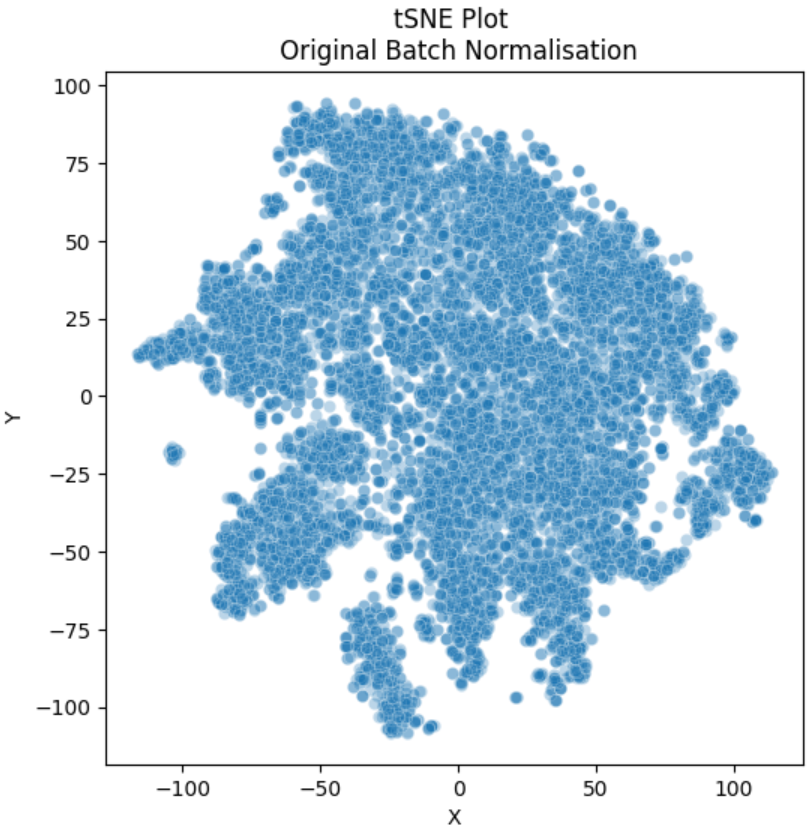
\includegraphics[width=0.49\textwidth]{original_bn}
		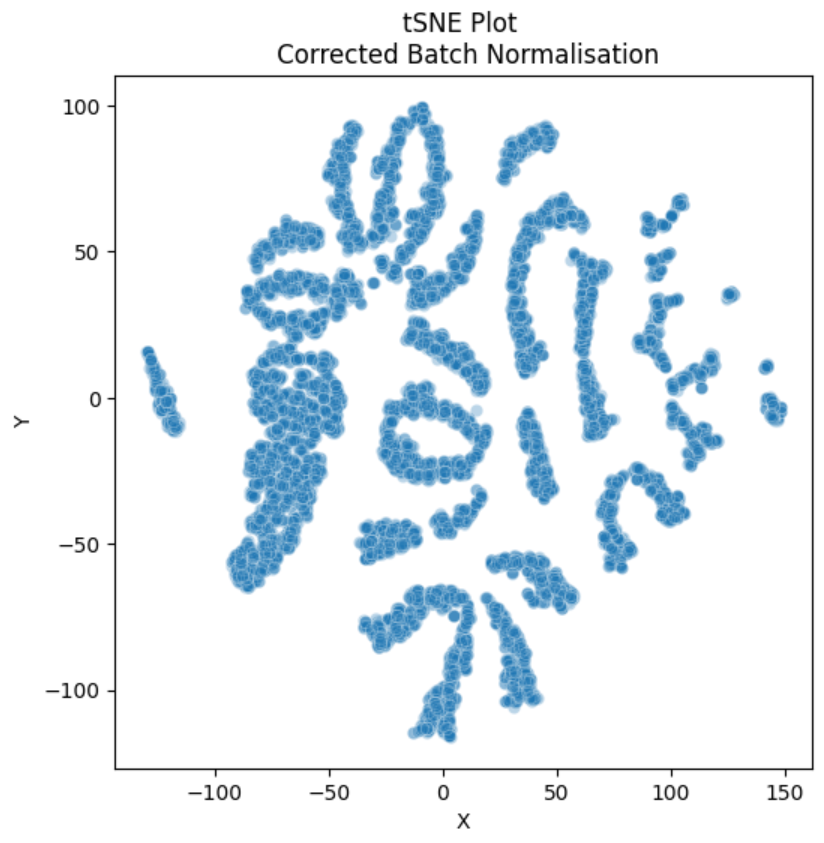
\includegraphics[width=0.5\textwidth]{bn}		
	\end{figure}
\end{frame}

\begin{frame}
	\frametitle{GNNs Embeddings}
	\begin{block}{Clusters' Properties}
		Below, the embedded space is colour-coded based on the molecules' ``acceptor'' and ``hydrophobe'' features. We can see the clusters are more or less similar. Also, it is interesting to see some hand-selected ions embedded closely in this space on the middle right side of the plots.
	\end{block}
	
	\begin{figure}
		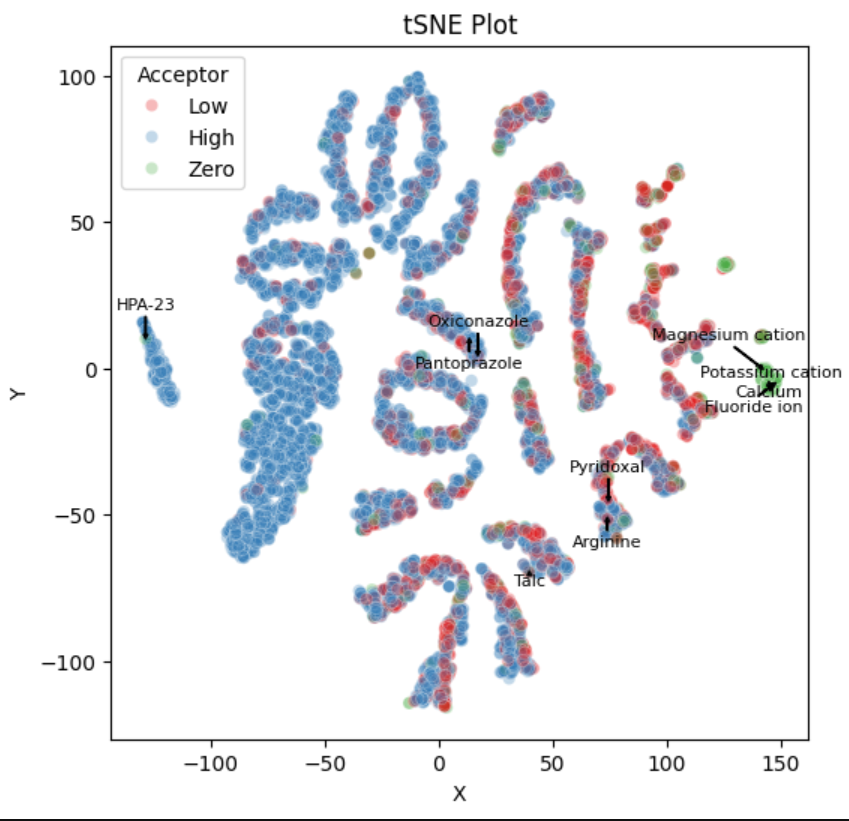
\includegraphics[width=0.49\textwidth]{acceptor}
		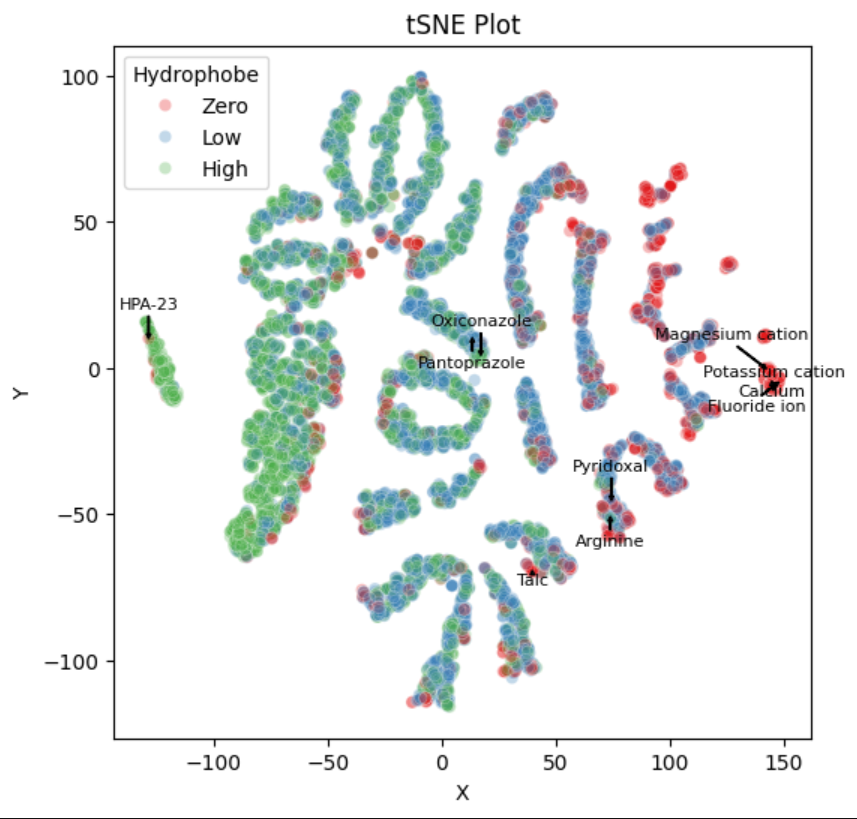
\includegraphics[width=0.5\textwidth]{hydrophobe}		
	\end{figure}
\end{frame}

\setbeamerfont{block body}{size=\small}

\begin{frame}
	\frametitle{GNNs Embeddings}
	\begin{block}{Discussion and Future work}
		\begin{itemize}
			\item Although the embedding space shows some merits regarding the similarity of close points, there is no reason to assume it can achieve a high score in the RAIDEN test since the original embedding was trained for a similar but not necessarily same downstream task.
			
			\item If we do not achieve an appropriate score, combining the current embedding architecture and the RAIDEN as the downstream task in the training phase can improve the embedding quality.
			
			\item A new idea for future work can be the introduction of molecular space similarity in an unsupervised fashion. For example, in \cite{zitnik_2017}, the author proposed a multi-layer network of different GNNs representing a tissue-specific protein-protein interaction. The tissue network ``uses a hierarchy to model dependencies between protein graphs'' \cite{zitnik_2017}.
						
			\item Domain knowledge about possible use cases for the downstream tasks (e.g., RAIDEN) can be incorporated by creating a hierarchy model based on the molecule features we think are relevant to the task.
		\end{itemize}
	\end{block}	
\end{frame}

\begin{frame}
	\frametitle{}
		\begin{block}{References}   
			\bibliographystyle{unsrt}
			\bibliography{cites}{}      
       \end{block}

      
\end{frame}


\end{document}